\thispagestyle{plain}
\section{Fracciones y decimales}
En esta sección, estudiaremos las fracciones y los decimales, que son dos formas de representar números racionales. Los números racionales son aquellos que se pueden expresar como el cociente de dos números enteros. Por ejemplo, $\frac{1}{2}$, $5$ o $7.6$. En esta sección, aprenderemos a representar números racionales en forma de fracción, en forma decimal y de forma entera. También aprenderemos a comparar fracciones, decimales y enteros, y a convertir de una forma a otra.

\subsection{Equivalencias de fracciones y decimales}

\subsubsection{Fracciones equivalentes}
Cuando dos fracciones representan el mismo número, decimos que son equivalentes. Por ejemplo, $\frac{1}{2}$ y $\frac{2}{4}$ son equivalentes, porque representan el mismo número. Para verlo, podemos dividir una pizza en dos partes iguales, y luego dividir una de esas partes en dos partes iguales.

Aquí podemos notar que $\frac{1}{2} = \frac{2}{4}$, y que $\frac{2}{4} = \frac{4}{8}$.

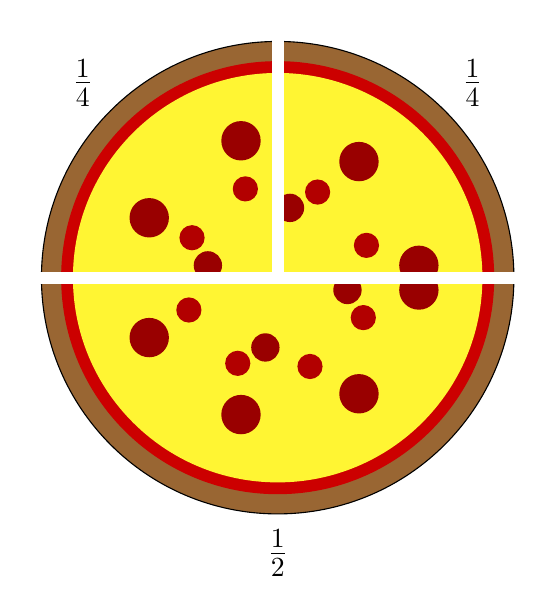
\begin{tikzpicture}
    % Crust
    \draw[fill=brown!80!black] (0, 0) circle (3cm);
    % Tomato Sauce
    \fill[red!80!black] (0, 0) circle (2.75cm);
    % Cheese
    \fill[yellow!80!white] (0, 0) circle (2.6cm);
    % Pepperoni
    \foreach \x in {5,55,...,365}
    \fill[red!60!black] (\x:1.8cm) circle (0.25cm);
    \foreach \x in {-10,80,...,305}
    \fill[red!60!black] (\x:0.9cm) circle (0.18cm);
    \foreach \x in {-25,20,...,290}
    \fill[red!70!black] (\x:1.2cm) circle (0.16cm);
    % Division lines for pizza slices
    \foreach \x in {0,90,180}
    \draw[line width=0.15cm, color=white] (0, 0) -- (\x:3.1cm);
    % Fractions labels
    \foreach \angle/\label in {45/4, 135/4
            , 270/2}
    \draw (\angle:3.5cm) node {\Large \bfseries $\frac{1}{\label}$};
\end{tikzpicture}
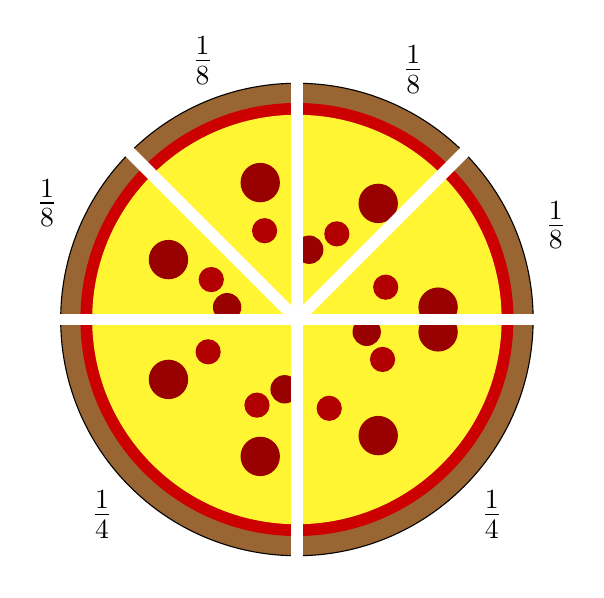
\begin{tikzpicture}
    % Crust
    \draw[fill=brown!80!black] (0, 0) circle (3cm);
    % Tomato Sauce
    \fill[red!80!black] (0, 0) circle (2.75cm);
    % Cheese
    \fill[yellow!80!white] (0, 0) circle (2.6cm);
    % Pepperoni
    \foreach \x in {5,55,...,365}
    \fill[red!60!black] (\x:1.8cm) circle (0.25cm);
    \foreach \x in {-10,80,...,305}
    \fill[red!60!black] (\x:0.9cm) circle (0.18cm);
    \foreach \x in {-25,20,...,290}
    \fill[red!70!black] (\x:1.2cm) circle (0.16cm);
    % Division lines for pizza slices
    \foreach \x in {0,45,...,180,270}
    \draw[line width=0.15cm, color=white] (0, 0) -- (\x:3.1cm);
    % Fractions labels
    \foreach \angle/\label in {20/8, 65/8,110/8, 155/8
            , 225/4,315/4}
    \draw (\angle:3.5cm) node {\Large \bfseries $\frac{1}{\label}$};
\end{tikzpicture}


% Representacion detallada en Tikz de una pizza de peperoni.
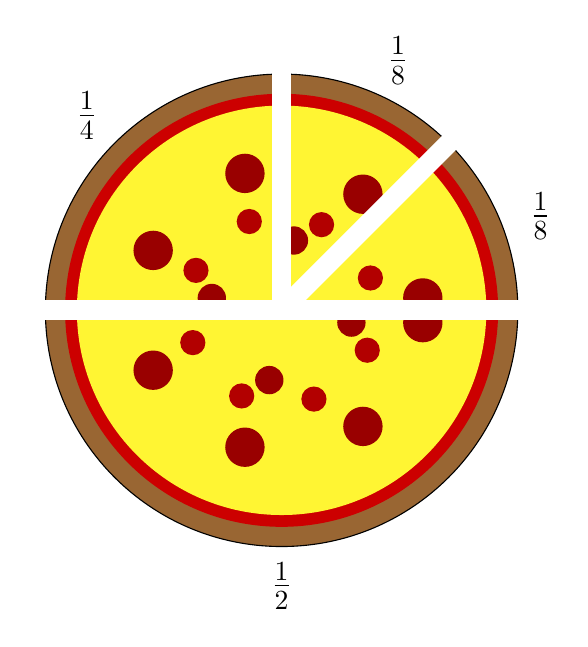
\begin{tikzpicture}
    % Crust
    \draw[fill=brown!80!black] (0, 0) circle (3cm);
    % Tomato Sauce
    \fill[red!80!black] (0, 0) circle (2.75cm);
    % Cheese
    \fill[yellow!80!white] (0, 0) circle (2.6cm);
    % Pepperoni
    \foreach \x in {5,55,...,365}
    \fill[red!60!black] (\x:1.8cm) circle (0.25cm);
    \foreach \x in {-10,80,...,305}
    \fill[red!60!black] (\x:0.9cm) circle (0.18cm);
    \foreach \x in {-25,20,...,290}
    \fill[red!70!black] (\x:1.2cm) circle (0.16cm);
    % Division lines for pizza slices
    \foreach \x in {0,45,90,180}
    \draw[line width=0.25cm, color=white] (0, 0) -- (\x:3.1cm);
    % Fractions labels
    \foreach \angle/\label in {20/8, 65/8, 135/4
            , 270/2}
    \draw (\angle:3.5cm) node {\Large \bfseries $\frac{1}{\label}$};
\end{tikzpicture}

% explicación de la equivalencia al entero de fracciones
\subsubsection{Equivalencias al entero}
Una fracción es equivalente al entero cuando el numerador es igual al denominador. Por ejemplo, $\frac{3}{3}$ es equivalente a $1$, porque
\begin{multicols}{2}
    \fracgraph{5}{2/cyan!50,3/red!40,4/brown!50}

    \begin{align*}
        \color{cyan!80!black}\dfrac{1}{2}+\dfrac{1}{2}                            & =\dfrac{2}{2}=1 \\[0.5em]
        \color{red!80!black}\dfrac{1}{3}+\dfrac{1}{3}+\dfrac{1}{3}                & =\dfrac{3}{3}=1 \\[0.5em]
        \color{brown!80!black}\dfrac{1}{4}+\dfrac{1}{4}+\dfrac{1}{4}+\dfrac{1}{4} & =\dfrac{4}{4}=1
    \end{align*}
\end{multicols}

\subsubsection{Convierte fracciones a decimales}
Para convertir una fracción a decimal, dividimos el numerador entre el denominador. Por ejemplo, para convertir $\frac{3}{4}$ a decimal, dividimos $3$ entre $4$.
\begin{center}
    \longdivision{3}{4} \qquad entonces, $\dfrac{3}{4}=0.75$
\end{center}

\subsubsection{Convierte decimales a fracciones}
Para convertir un decimal a fracción, debemos escribir el número decimal como una fracción decimal, y luego simplificarla. Por ejemplo, para convertir $0.75$ a fracción, escribimos $0.75$ como $\frac{75}{100}$, y luego simplificamos la fracción.
\[0.75=\frac{75}{100}\]
En una \textbf{fracción decimal} el denominador debe ser una potencia de $10$. En este caso, el denominador es $100$, que es una potencia de $10$. Si el decimal tiene un solo dígito después del punto decimal, el denominador debe ser $10$. Por ejemplo, para convertir $0.5$ a fracción, escribimos $0.5$ como $\frac{5}{10}$, y luego simplificamos la fracción.
\[0.5=\frac{5}{10}\]
Para \textbf{simplificar una fracción}, dividimos el numerador y el denominador entre el máximo común divisor de ambos. En este caso, el máximo común divisor de $75$ y $100$ es $25$, por lo que la fracción simplificada es
\[\frac{75}{100}=\frac{75\div25}{100\div25}=\frac{3}{4}\]

\subsection{Decimales peri\'odicos}
Un decimal periódico es un decimal que tiene un patrón de dígitos que se repite infinitamente. Por ejemplo, al convertir la fracción $\frac{1}{3}$ a un número decimal, se obtiene:
\begin{center}
    \longdivision[stage=1,repeating decimal style = none]{1}{3}
\end{center}
$0.3333\dots$ es un decimal periódico, porque el patrón $3$ se repite infinitamente. El patrón de un decimal periódico se llama \textbf{período}. El período de $0.3333\dots$ es $3$, y se escribe como:
\[0.3333\dots=0.\overline{3} \qquad \text{(Se pronuncia ``\emph{cero punto tres periódico}'')}\]

\subsubsection{Redondeo y truncamiento}
Cuando convertimos una fracción a decimal, a veces obtenemos un decimal que no termina nunca de escribirse por completo. Por ejemplo, al convertir $\frac{1}{3}$ a decimal, obtenemos $0.3333\dots$. En este caso, podemos \textbf{redondear} el decimal a un número finito de dígitos, o podemos \textbf{truncar} el decimal a un número finito de dígitos.

\paragraph{Redondeo} Redondear un número quiere decir reducir el número de cifras manteniendo un valor parecido. El resultado es menos exacto, pero más fácil de usar. Para redondear un decimal, debemos decidir cuántos dígitos queremos en el resultado. Luego, miramos el siguiente dígito después del último dígito que queremos en el resultado. Si el siguiente dígito es $5$ o más, sumamos $1$ al último dígito que queremos en el resultado. Si el siguiente dígito es menor que $5$, no sumamos nada al último dígito que queremos en el resultado.

Por ejemplo, para redondear $0.6666\dots$ a $2$ dígitos, miramos el tercer dígito, que es $6$. Como $6$ es mayor que $5$, sumamos $1$ al segundo dígito, y obtenemos $0.67$.

https://www.expii.com/t/rounding-decimals-definition-examples-9071

Redondea 6,121.87856 a la milésima más cercana.
Paso uno: Identifique el dígito en el valor posicional dado. Desde nuestro decimal
es 6,121.87856 , el número en el lugar de las milésimas es 8:
\[6,121.87\boxed{8}56\]


Paso dos: identifica el dígito al lado. El dígito al lado del 8 en el
lugar de las milésimas es 5:
\[6,121.87 \boxed{8} \boxed{5} 6\]

Paso tres: redondea el nuevo número (el compuesto por los dígitos del Paso
Uno y Paso Dos) a la decena más cercana. Este nuevo número es 85, que obtuvimos
del 8 en el paso uno y del 5 en el paso dos:
\[6,121.87 \boxed{85} 6\]
Cuando redondeamos a la decena más cercana, obtenemos 90:
\[6,121.87 \boxed{90} 6\]
Paso cuatro: ¡Elimine todos los dígitos después del valor posicional dado! Recuerda, nuestro
el valor posicional dado era el lugar de las milésimas. Cuando eliminamos todos los dígitos después
el 9 en el lugar de las milésimas, obtenemos:
\[6,121.879\]

Redondear un número es una forma de hacer que un número sea menos exacto al comvertirlo
en una estimación.

¿Por qué querrías que un número fuera menos preciso?, podrías preguntar. Para principiantes,
Los números redondeados son fáciles de hacer con los cálculos. Es mucho más fácil agregar,
\[300 + 500\],
que sumar,
\[312 + 498\]
Otras veces simplemente no necesitas precisión. Si fuiste a un concierto, no necesitas decir que había 399,342 personas
en el estadio. Simplemente diría que había alrededor de 400,000.

Para redondear decimales, primero debe asegurarse de conocer su lugar valores. En su mayoría, se le pedirá que redondee un número a un valor posicional específico. Para hacer esto, mira el número a la derecha del valor posicional. Si es un 5 o más, eleva el número en el valor posicional en uno. Si se
es un 4 o menos, deja el número solo en el valor posicional. Una vez que hagas esto,
convierte todos los dígitos a la derecha del valor posicional en 0.

Supongamos que queremos aproximar 42.49275 a la milésima más cercana.

Primero se localiza el valor posicional dado. En este caso, milésimas.
\[42.49\boxed{2} 75\]

A continuación, miramos el dígito a la derecha.
\[42.49\boxed{2} \boxed{7}5\]

Aquí, es 7. Como esto es mayor que 5, aumentamos el número del valor posicional en uno.
\[42.49\boxed{3} \boxed{0}5\]
Finalmente, eliminamos todos los dígitos a la derecha del valor posicional.
\[42.49\boxed{3} \]


Ahora supongamos que queremos redondear 42.09998 a la diezmilésima más cercana.

Ubicando el valor posicional encontramos al digito 9.
\[42.099\boxed{9} \boxed{8}\]
El número a su derecha, 8, que es mayor que 5 por lo que aumentamos nuestro valor posicional en uno. Pero
esto convierte nuestro 9 en un 10. Convierte el 9 en un 0 y aumenta
el siguiente dígito a la izquierda en uno. Esto convertirá cualquier 9 seguido en 0
finalmente aumentando décimas en uno.
\[42. \boxed{100}\boxed{0}\boxed{8}\]
Finalmente, eliminamos cualquier dígito a la derecha de nuestro valor posicional.
\[42.100\]
Podemos omitir cualquier exceso de ceros.
\[42.1\]

En el caso especial en el que queremos redondear al número entero más cercano,
no habrá nada después del punto decimal una vez que hayamos terminado.

Redondear decimales funciona igual que redondear números enteros.

Para redondear un decimal a un valor posicional dado, mire el dígito en el lugar
A la derecha.

Si el dígito es menor que 5, se redondea hacia abajo. Si el dígito es mayor que
o igual a 5, se redondea hacia arriba. Por ejemplo, redondeemos 1.41 al más cercano
décimos Seleccionemos el dígito de las décimas, 4, con azul.
\[1. {\color{blue!80!black} 4 } 1\]

A continuación, seleccione el dígito a la derecha.
\[1. {\color{blue!80!black} 4 } {\color{green!80!black} 1 }\]

Como 1 es menor que 5, vamos a redondear hacia abajo. Dejamos 4 tal cual y
haga que todos los dígitos a la derecha sean 0.
\[1. {\color{blue!80!black} 4 } {\color{green!80!black} 0 }\]

\paragraph{Truncamiento} Para truncar un decimal, debemos decidir cuántos dígitos queremos en el resultado. Luego, eliminamos todos los dígitos después del último dígito que queremos en el resultado.
Por ejemplo, para truncar $0.6666\dots$ a $2$ dígitos, eliminamos todos los dígitos después del segundo dígito, y obtenemos $0.66$.

\newpage